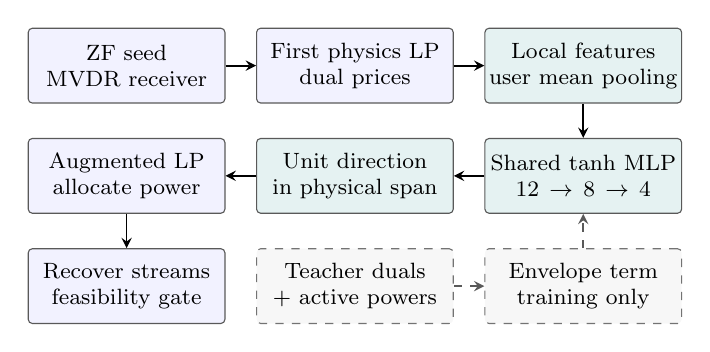
\begin{tikzpicture}[
    x=1mm,y=1mm,
    font=\footnotesize,
    block/.style={draw=black!65,rounded corners=1.5pt,align=center,
        text width=24mm,minimum height=9.5mm,inner sep=1.4pt,fill=white},
    physics/.style={block,fill=blue!5},
    learned/.style={block,fill=teal!10},
    training/.style={block,draw=black!55,dashed,fill=black!3},
    flow/.style={->,>=stealth,line width=.65pt},
    supervise/.style={flow,dashed,draw=black!65}
]
\node[physics] (seed) at (0,0) {ZF seed\\MVDR receiver};
\node[physics] (first) at (29,0) {First physics LP\\dual prices};
\node[learned] (features) at (58,0) {Local features\\user mean pooling};
\node[learned] (net) at (58,-14) {Shared tanh MLP\\\(12\to8\to4\)};
\node[learned] (beam) at (29,-14) {Unit direction\\in physical span};
\node[physics] (next) at (0,-14) {Augmented LP\\allocate power};
\node[physics] (recover) at (0,-28) {Recover streams\\feasibility gate};
\node[training] (teacher) at (29,-28) {Teacher duals\\+ active powers};
\node[training] (loss) at (58,-28) {Envelope term\\training only};
\draw[flow] (seed) -- (first);
\draw[flow] (first) -- (features);
\draw[flow] (features) -- (net);
\draw[flow] (net) -- (beam);
\draw[flow] (beam) -- (next);
\draw[flow] (next) -- (recover);
\draw[supervise] (teacher) -- (loss);
\draw[supervise] (loss) -- (net);
\end{tikzpicture}
